\chapter{Beamline}

The Hall~C beam line transfers beam from the extraction line to the Hall~C target.

\section{Beamline}

It executes the following functions:

\begin{itemize}
\item{Provide a fine waist focusing on the target.}
\item{Beam energy, beam energy spread, and beam emittance measurements
in the arc section.}
\item{Vertical chicane beam transfer for the polarized target.}

\item{High precision beam angle measurement for selected cross section
experiments.}
\end{itemize}

\subsection{Control}

All magnets (dipoles, quads, sextupoles, beam
correctors) and beam diagnostic devices (BPM, harp, BCM, viewer)
are controlled by machine control center (MCC) through EPICS,
except for a few special elements, which are addressed in the
subsequent Sections.

\subsection{Monitoring}
To start up the beam position monitor (BPM) and beam current monitor
(BCM) displays which are normally displayed continuously on X-terminal
HALLCXT9, do these steps:
\begin{itemize}
  \item {as cvxwrks on cdaqh1, run \verb|medm|.}
  \item {click \verb|execute|.}
  \item {{\em For BPM}open \verb|MEDM/bpm/gueye/hcbpms_gueye_jan99.adl|}
  \item {{\em For BCM}open \verb|MEDM/saw/bcm.adl|}
\end{itemize}
  

\subsection{Safety procedures}

Detailed safety procedures are specified in the following documents:

\begin{itemize}
\item{Fast shut down system}
\item{MCC emergency plan}
\item{Incident-response procedure}
\item{Safety systems reference and procedure}
%\item{Search and secure procedure}
%\item{Electrical-hazard testing procedure}
%\item{Entry requirements}
%\item{Safety inspection checklists}
%\item{PSS interlock}
%\item{Radiation exposure emergency response procedure}
\end{itemize}

\subsection{Machine/Beam line protection system}

The MPS system is composed of the fast shutdown (FSD), beam loss
monitor (BLM), beam loss accounting (BLA), and gun control systems.

The FSD system is a network of permissive signals which terminate
at the electron gun. The permissive to the gun may be inhibited by any 
device connected to an FSD node.
Devices connected to the FSD system include vacuum valves, RF
systems, beam loss systems, beam current monitors, and beam dumps.

The gun control system includes software program which monitor
beam operating conditions and the state of the FSD, BLM, and BLA systems.
The program will warn the operators if a potential for beam damage
exists. Potential for damage exists when running high average current
beam, when FSD nodes are masked, and when the beam power approaches
the operating envelope limits for a specific beam dump.

\subsection{Reference documents}

The following Reference Documents are available:

\begin{itemize}
\item{Accelerator Operations Directives, May 9, 1994}
\item{Tunnel song sheet and drawings, June 25, 1995}
\item{Hall~C beam line elements list, June 9, 1994}
\item{Hall~C team summary notebook}
\item{Hall~C beam line commissioning procedure, May 1995}
\item{Hall~C beam energy measurement commissioning procedure, June 22, 1995}
\end{itemize}

\section{Special Beam Line Elements}

There are several special beam line elements which were temporarily
controlled by the Hall~C group. We transfered them to machine
control center in 1996 when the R\&D period was over.

Those special beam line elements include:  raster systems; superharp systems; the M\o ller 
Polarimeter; the bremsstralung radiator; and current measuring devices.

\subsection{Raster Systems}

Vertical and horizontal air-core magnets provide beam
rastering patterns on the Hall~C target (Fast Raster or FR), the
Hall~C M\o ller Polarimeter target (M\o ller Raster or MR), and the Hall~C 
Polarized Target Raster (SR) in order to prevent possible damage to the material by
overheating. All are AC magnets. No DC fields 
exist when they are operated. No remanent field remains after
the current is switched off.

Both FR and SR magnets are driven by a 250 W audio amplifier. The FR
and SR magnets are shielded by a plexiglass cage and are marked with a
``high voltage dangerous'' symbol.  A red light indicates the
operation of these two raster systems. During their operation, personnel
should be away from the resonance loop because the rms voltage across
the magnets is over 400 V.

The M\o ller raster magnets are located on the accelerator side of the
beamline shield wall.

The following conditions lead to a fast shutdown of the raster devices:
\begin{itemize}
\item{Crate power failure}
\item{Magnets power failure}
\item{Overcurrent detection (short occurs inside the magnets)}
\item{Over temperature}
\item{Detection of missing cycles or improper frequency}
\item{VME system reset}
\item{Phase-lock network is broken}
\end{itemize}

\noindent Both FR and SR power drivers have an automatic fault display and
shutdown. The signals are also sent to FSD.

The following Reference Documents exist:
\begin{itemize}
\item{Requirement for beam raster monitor for the beam dump and target,
R. C. Cuevas, C. Yan, 12 July, 1995}
\item{Technical requirement for Hall~C beam dump raster,
C. Yan, June 24, 1995, JLab-R-94-02}
\item{M\o ller Raster Manual at \verb|~cdaq/documents/beamline/Moller_Raster_Manual.txt|}
\end{itemize}

\subsection{Superharp Systems}

The superharp systems are mainly used for beam energy measurement,
but are also used as a reference for BPM calibration, and as
normal beam profile monitors for machine operation. Three pairs
of superharps are located on the pre-aligned granite tables at the
beginning, the mid-point, and the end of arc.
Separate superharps are located in combination with BPM's in the
Hall~C beamline segment close to the Hall~C target.

When the Hall~C arc is tuned in the so-called ``dispersive" mode
the three pairs of superharps are successively operated to obtain
the positions and orientations of the incident and outgoing beam,
which renders also the central trajectory. The combination of
beam positions and beam profile as given by the three superharp
pairs, together with the known field integral of the arc bend
magnets, can be used to derive the beam energy and also the beam
emittance and dispersion.

Anyone who has access to enter the Hall~C beam line tunnel should
not bump the three granite tables because the superharp
crosses are aligned with high precision. Any beam line work in this
section should be discussed with the JLab survey group in advance.

Superharp operation is shared by Hall~C and MCC. To prevent any
disturbance of software an authorized path and area must be
installed for its secure operation. Anyone (including Hall~C persons
and users) who wants to change directory or reboot IOC should
report to the responsible personnel
in advance.

With the normal scan velocity setting of 20000 Steps per second, the
maximum cw current that the 22 micron tungsten wire can stand is about
20 $\mu$A. Above this value superharp operation is prohibited.

The following Reference Documents are available:
\begin{itemize}
\item{JLab-R-94-01}
\item{JLab HARP record detailed design document, D. Barker, May 31, 1994}
\item{Hall~C requirements for the superharp scanning system, D.
Barker, C. Yan}
\end{itemize}


\paragraph{The Superharp Device}\label{system}

The superharp consists of a wood fork holding a 22~$\mu$m tungsten wire segmented in three
perpendicular sections. This fork can be inserted in and out of the beam pipe, causing an
interaction between the wires and the electron beam (Fig.~\ref{figure:superharp}).


\begin{figure}[!hbt]
\begin{center}
%\htmlimage{flip=r270}
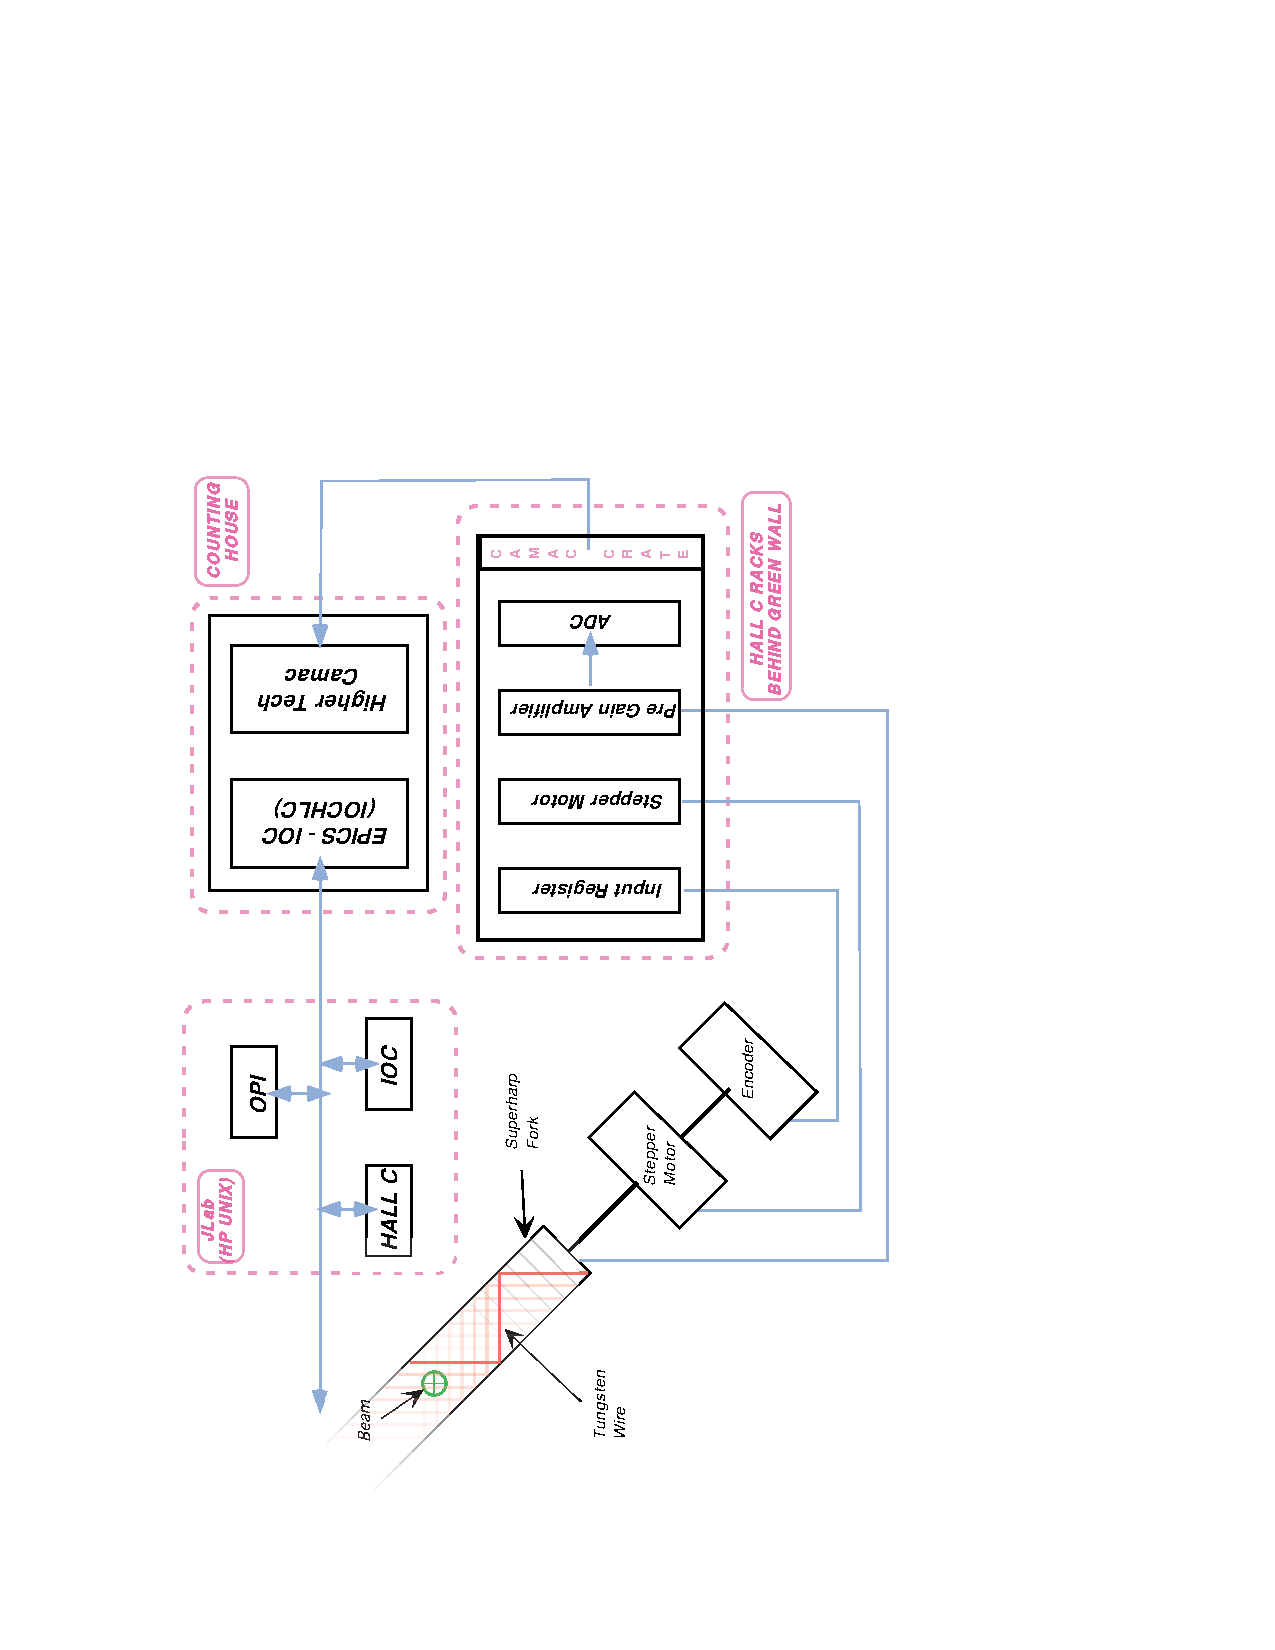
\includegraphics[width=6in,angle=270]{beamline/superharp-system.ps2}
\caption{Schematic of the superharp system.}
\label{figure:superharp}
\end{center}
\end{figure}

The horizontal and vertical positions of the beam are then determined by collecting the charges
produced as the wires go through the electron beam within an accuracy of about 
%!!! $\pm 50~\mu$m
(see Fig.~\ref{figure:interface} in section~\ref{interface}). While the superharp fork
is travelling inside the beam pipe, three diferent signals appears due to the interaction
between the JLab beam and each of the three wires. The time duration during a scan is
approximately 30~sec from the starting rest position to the maximum allowed travel distance
(about 3''=7.62~cm).

The signals are then sent to an Analog Digital Converter (1881-ADC) electronic card and then transfered
to a computer for data analysis. Due to the interaction beam-wires, this device spreads the beam
(destructive method). In addition, with the information on the horizontal position inside the arc, the
energy of the electron beam can also be monitored~\cite{Gueye-98-energy}. This feature will be described
later in section~\ref{analysis}. The current range for these wires is
between 1 and 30~$\mu$A.  

Since some experiments in hall C will run with a current below
1~$\mu$A,  some BLMs have been added to the
current electrode channels.

The Beam Loss Monitor (BLM) is a photo-multiplier tube (Hamamatsu-931B, side cathode) which detects
particles produced when the wires from the superharp's fork interacts
with the  electron beam. Each
superharp has one BLM located downstream about 10~cm (target) and
0.5-2~m ( hall C arc). Combined with
the electrode channel, the total current range of a single superharp device is
$0.01 < I~(\mu {\rm A}) < 30$.

\paragraph{The superharp interface window}\label{interface}

The automated hall C superharp interface window program allows control of both
data acquisition and data analysis. The flow chart of the code is shown on Fig.~\ref{figure:flow_chart}. 
Each superharp device is controlled via 
\htmladdnormallinkfoot{EPICS}{http://epics.aps.anl.gov/asd/controls}. The
signals obtained from a scan are then
stored into an ASCII file which serves as an input file for a {\tt C++} routine where all the
calculations are performed. The main interface window is shown on Fig.~\ref{figure:interface}.

\begin{figure}[!hbt]
\begin{center}
%\htmlimage{thumbnail=0.5,scale=1.0}
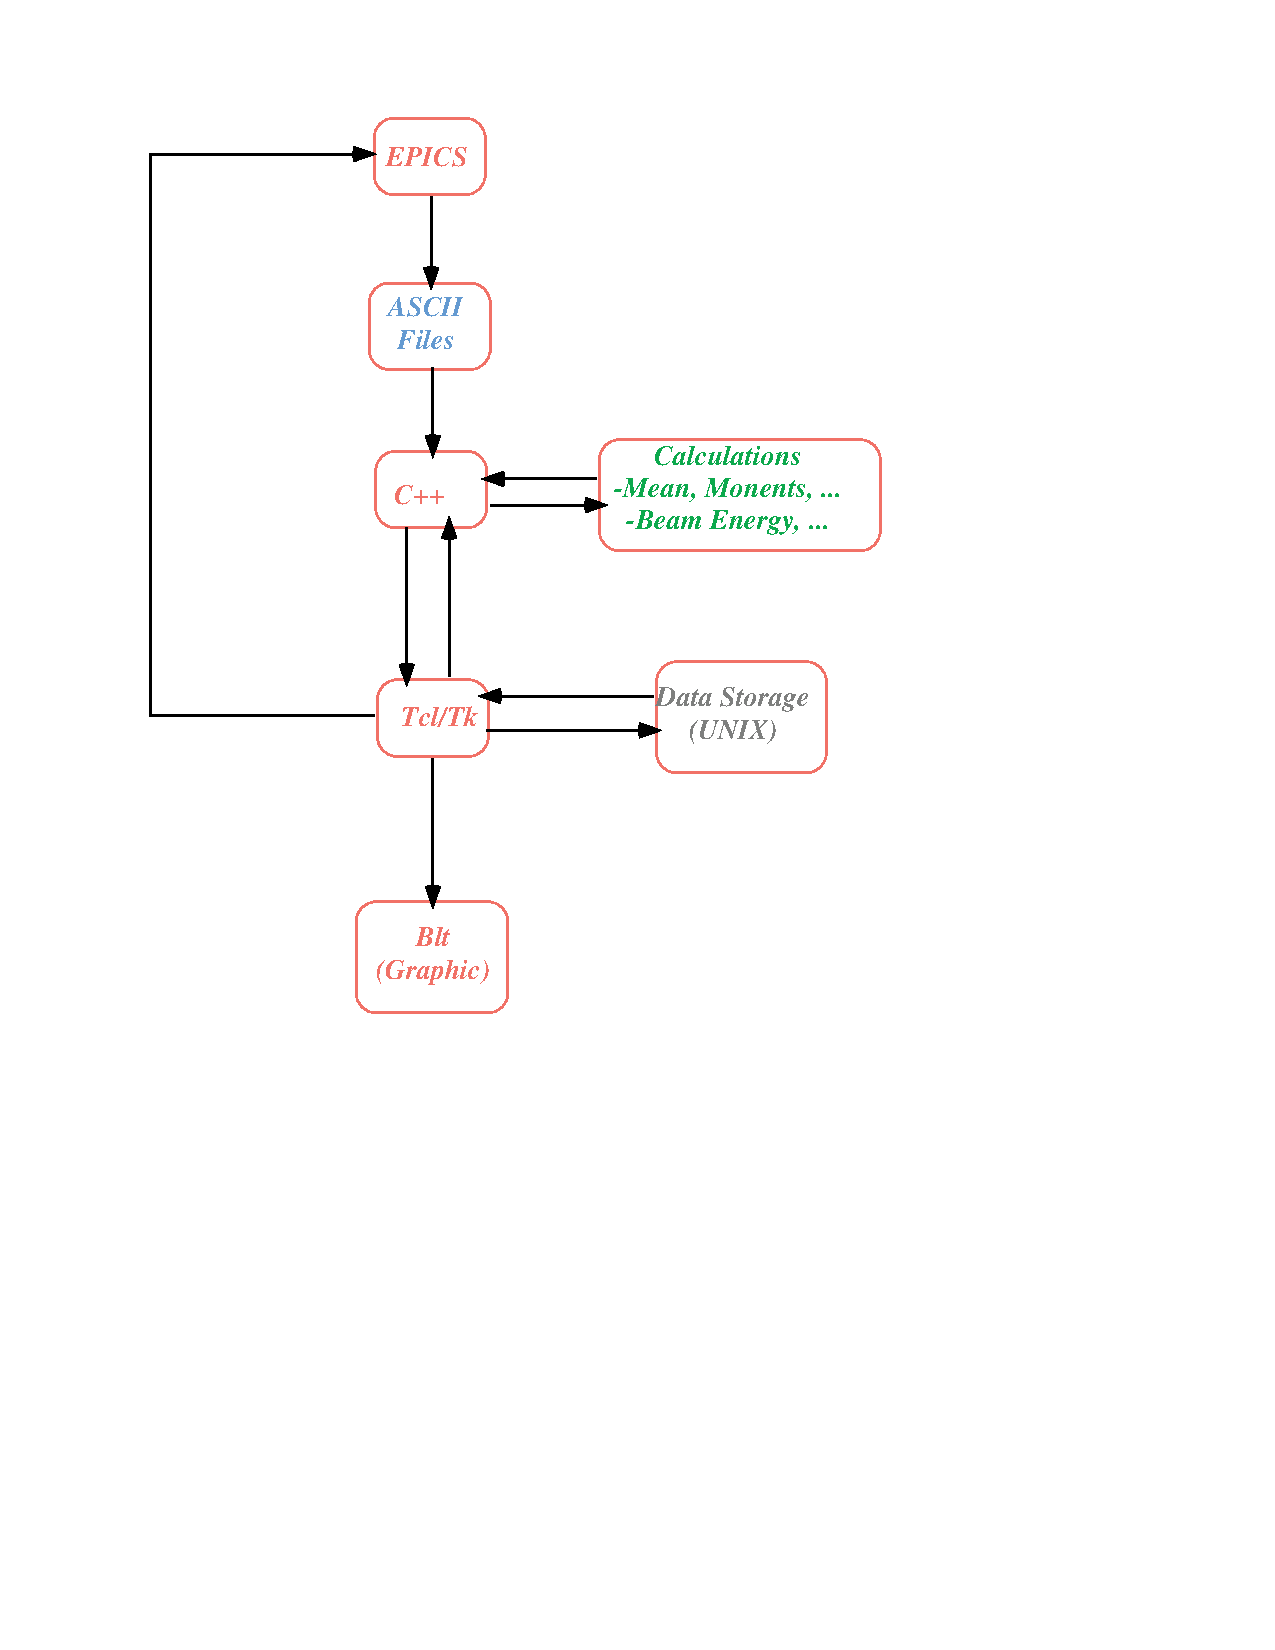
\includegraphics{beamline/superharp-flowchart.ps2}
\caption{Flowchart of the hall C superharp interface program.}\label{figure:flow_chart}
\end{center}
\end{figure}

%%note: natural size of following figure is 7wx8.85h inches.
\begin{figure}[!hbt]
\begin{center}
%\htmlimage{thumbnail=0.5,scale=4.0,flip=r270}
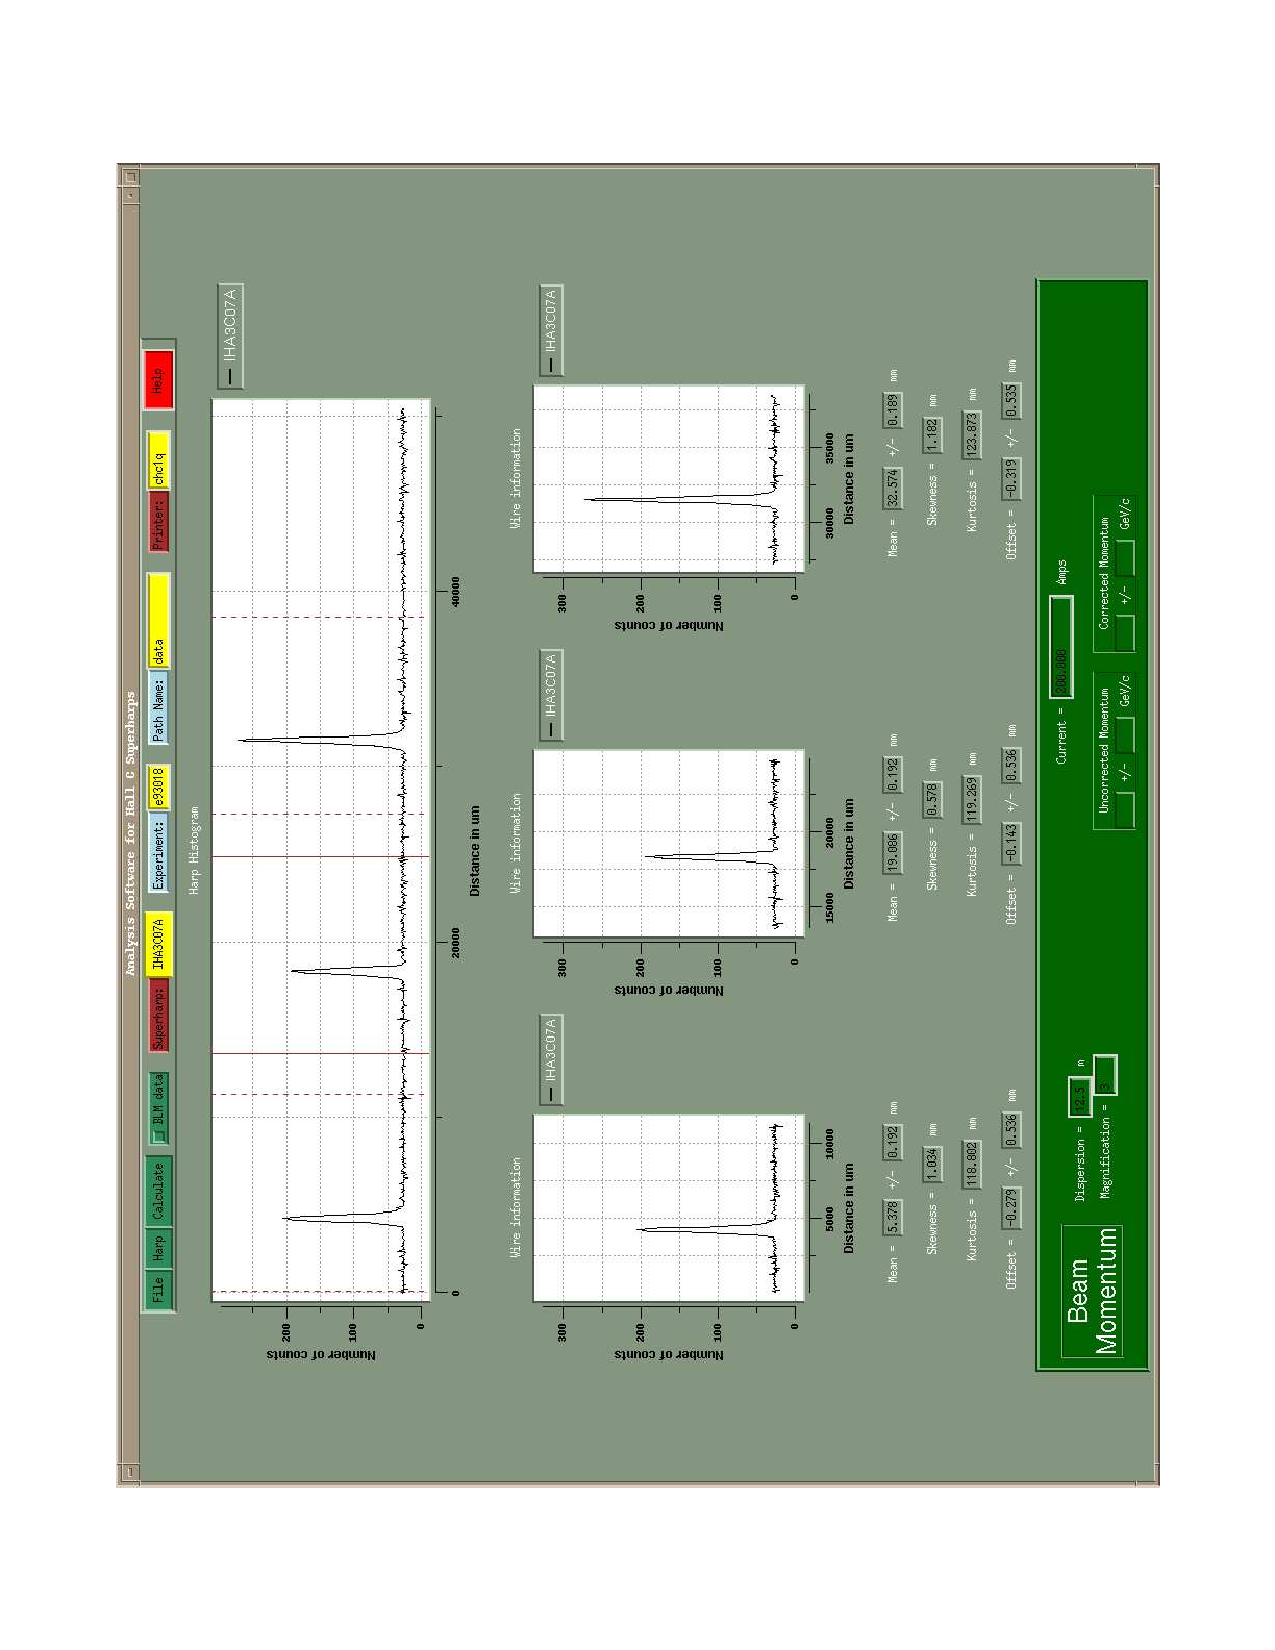
\includegraphics[height=6.5in,width=5.5in]{beamline/superharp_interface.ps2}
\caption{The hall C superharp interface window.}\label{figure:interface}
\end{center}
\end{figure}

In this section, we will review the different menu items that allow users to perform a scan and
perform data analysis.

	\subparagraph{Data Acquisition}\label{daq}

The corresponding code is running only on the actual {\bf cdaqh1} cluster located in the experimental
hall C counting house. Selecting {\bf\fbox{Harp $>$ Scan}} launches the {\tt MEDM} executable routine.

There are two control panels: one allows the user to select the appropriate superharp
(Fig.~\ref{figure:choose_harp}) and one to perform the scanning process (Fig.~\ref{figure:scan_harp}).

\begin{figure}[!hbt]
\begin{center}
%\htmlimage{thumbnail=0.5,scale=2.0}
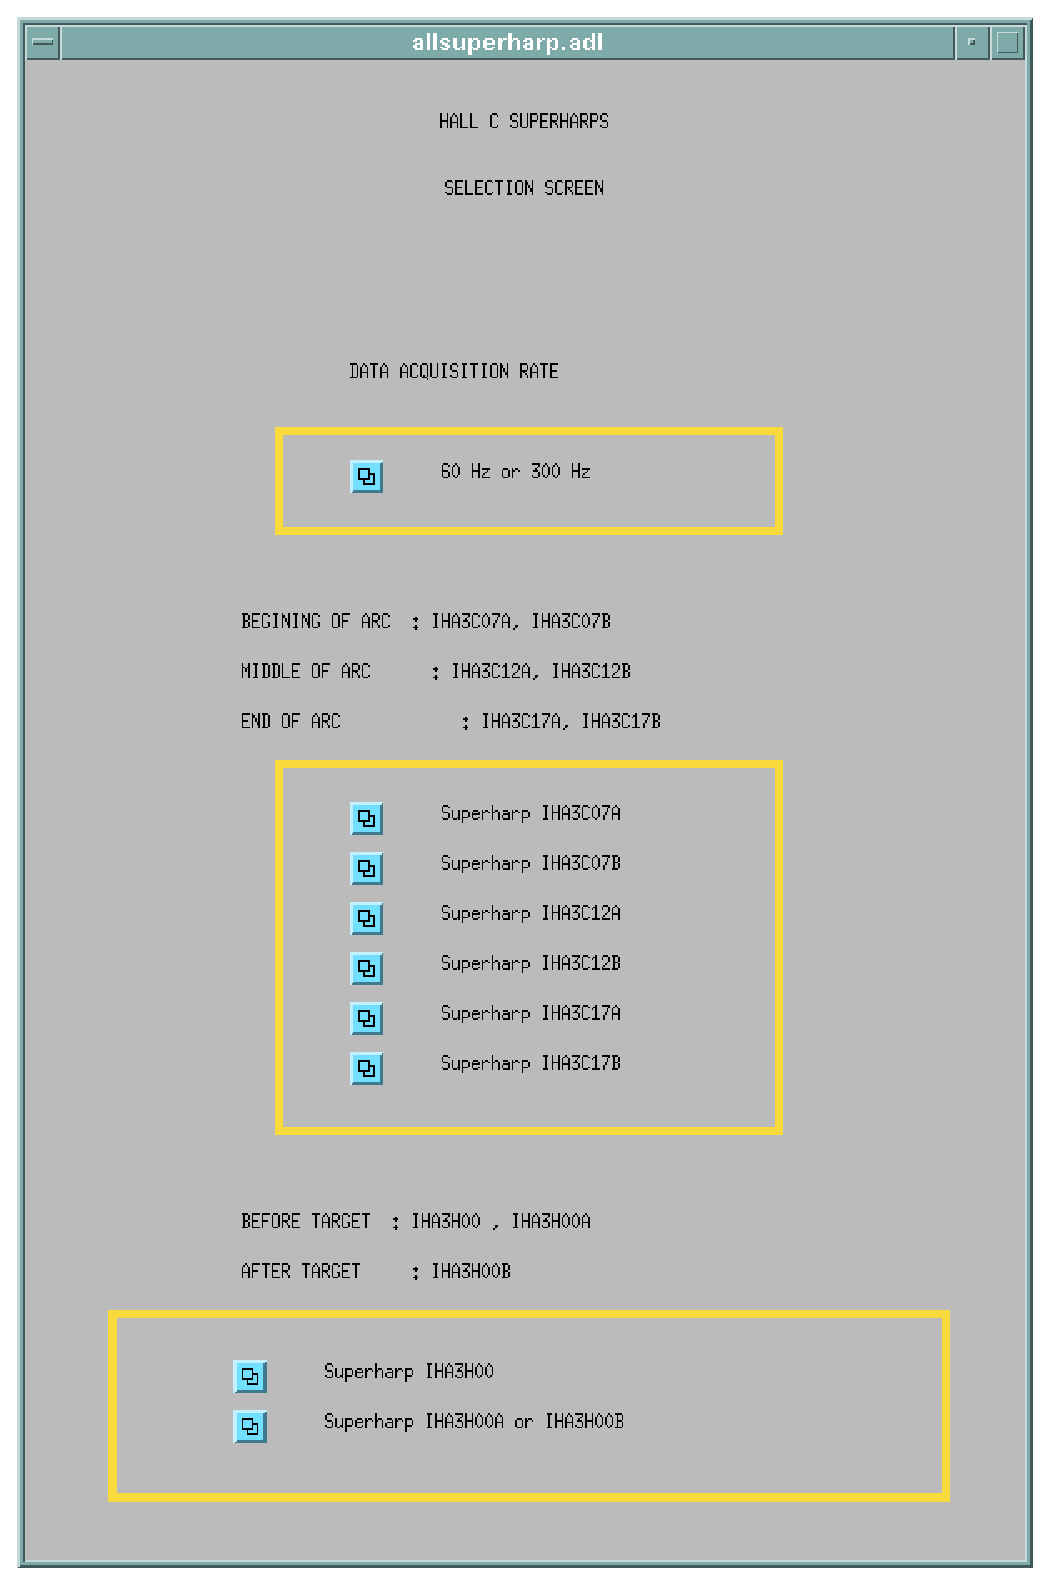
\includegraphics[height=7.2in]{beamline/superharpChoicePanel.ps}
\caption{The hall C superharp selection control panel.}\label{figure:choose_harp}
\end{center}
\end{figure}


\begin{figure}[!hbt]
\begin{center}
\includegraphics{beamline/scan-panel.eps}
\caption{The hall C superharp scanning control panel.}\label{figure:scan_harp}
\end{center}
\end{figure}

Before starting any scanning process, verify that you have the correct default parameters as shown in
Table~\ref{table:scan_harp} below.
\begin{table}[!hbt]
\begin{center}
\begin{tabular}{llr}
\hline
\hline
{\it Values:}			&	\\ 
Acceleration			& 2000~tr/min	\\
Velocity			& 20000~tr/min	\\
Deceleration			& 2000~tr/min	\\
Pre-Gain Amplifier (PGA)	& 2	\\
\hline
\hline
{\it Messages:} 		&	\\
State				& 1	\\
Status				& Declared Zero Point Harp Position \\
Input Register			& 64335 \\
Analog Digital Converter (ADC) counts& 10-30 (background) \\
Cmd Readback			& 129	\\
\hline
\hline
\end{tabular}
	\caption{The default scan parameters for the hall C superharp system.}
	\label{table:scan_harp}
\end{center}
\end{table}
If not, then enter the correct value(s) and hit {\bf\fbox{return}}. Note that the value will {\bf not}
change  unless you hit \fbox{\bf return}. The last two digits in the
{\bf\fbox{Input Register}} box may
not be the same due to the 10~$\mu$m accuracy of the encoder.

After launching {\tt MEDM}, click on the red {\bf\fbox{SCAN}} button to begin the scan. The list
below describes the  change in several important variables during the scanning process.
\begin{enumerate}
\item \fbox{{\bf State}} changes from 1 to 4.
\item \fbox{{\bf Status}} indicates {\it Harp is moving}, {\it Harp is retracting}, and
	{\it Declared zero harp position} during the corresponding motion of the harp.
	{\it Declared zero harp position} indicates that the scan is finished and the harp has
	returned to its fully retracted rest position.
\item \fbox{{\bf Velocity}} changes to 30000~tr/min when the harp comes back.
\item \fbox{{\bf ADC}} registers the number of electrons picked up when a wire crosses the beam.
\item \fbox{{\bf Cmd Readback}} reads {\bf 66} when the harp is moving in the forward direction
	and {\bf 65} in the backward direction.
\end{enumerate}


	\subparagraph{Data analysis}\label{analysis}

Although \fbox{\bf harp\_ana\_new} is the main executable, the files \fbox{\bf harp\_ana\_new.tk}
and \fbox{\tt bltwish} are both required: \fbox{\bf  harp\_ana\_new.tk} contains the graphical routines
for the program and is interpreted at run-time through \fbox{\bf bltwish}. \fbox{\bf harp\_ana\_new} contains
both {\tt C++} and {\tt Tcl/Tk} codes: \fbox{\bf harp\_ana\_new} is written in {\tt C++} and contains most
of the calculation routines, and \fbox{\bf  harp\_ana\_new.tk} is written in {\tt Tk} and contains the user
interface and graphing routines.

	\subparagraph{Menu and entry Items}

The menu commands and entry items are described in Table~\ref{table:menu_entry}.
\begin{table}
\begin{center}
\begin{tabular}{||l|c|l||}
\hline
\hline
\multicolumn{3}{|c|}{\bf Menu Commands and Accelerator}	\\
\hline
File Reset & Ctrl-R & Clears all graphs and removes all data. \\
File Load  & Ctrl-L & Load all data in the current path. \\
File Save  & Ctrl-S & Saves all data in the current path. \\
File Print & Ctrl-P & Prints all graphs to the current printer.\\
File Quit & Ctrl-Q & Exits the program. \\
\hline
Harp Options & & Calls the configuration dialog. \\
Harp Scan & & Launches the medm scanning routine. \\
\hline
Calculate dP/P0 & & Calculates $P$ and $\Delta P$ based on the current data. \\
Calculate Smooth & Ctrl-M & Filters out background noise in all graphs. \\
Calculate Unsmooth & Ctrl-U & Reverses Calculate Smooth. \\
Calculate Transform & Ctrl-T & Calculates the Fourier cosine transform \\
		& & of the data. \\
\hline
\hline
\multicolumn{3}{|c|}{\bf Entry Items}	\\
\hline
Superharp	& & Load the selected superharp from the path	\\
		& & listed in the {\it File Name} entry and graphs it		\\
Experiment	& & Specifies the number of the current experiment.	\\
		& & The destination for files created by File Save 	\\
		& & is {\tt scan\_data/}{\it{Experiment}}{\tt /}{\it File Name}	\\
File Name	& & Specifies the location of the harps to be loaded	\\
		& & or the destination for the files created			\\
		& & by File Save			\\
Printer		& & Specifies the current printer				\\
\hline
\hline
\end{tabular}
	\caption{Definition of the menu commands, accelerators and entry items.}\label{table:menu_entry}
\end{center}
\end{table}

	\subparagraph{Help and BLM data}

The two remaining buttons on the superharp interface window menu bar, \fbox{{\bf BLM data}} and
\fbox{{\bf Help}}, allow users to switch to the BLM channels and displays this document ({\tt harphelp.ps}),
respectively.

\paragraph{Using the Program}\label{program}

This section describes in detail how to use harp\_ana\_new to execute common commands.

	\subparagraph{Loading Old Harp Data}

Data is loaded by selecting the name of the harp from the {\it Superharp} drop-down menu.  The program
looks in the path {\tt scan\_data/}{\it Experiment}{\tt /}{\it File Name}, where {\it Experiment} is
the experiment number listed in the {\it Experiment} entry and {\it File Name} is the file name listed
in the {\it File Name} entry.

	\subparagraph{Loading New Harp Data}

Data collected through Options Scan is automatically converted into a format readable by
{\fbox{\bf harp\_ana\_new}}, so it can been loaded, even in the same session in which it was collected,
as if it were old harp data.

	\subparagraph{Graphing Old Harp Data}

Harp data is automatically graphed when loaded (by selecting it from the {\it Superharp} drop-down menu).
The statistical information for the first graph loaded is also displayed.

	\subparagraph{Graphing New Harp Data}

Connect to {\tt cdaqh1} and run \fbox{\bf harp\_ana\_new}.  Select \fbox{Options Scan}, and follow the
instructions in the {\tt MEDM} section to scan in new data.  After exiting {\tt MEDM}, the new data should
appear. Note that it takes about 10 to 15 seconds for {\tt MEDM} to load.

	\subparagraph{Saving Harp Data}

Selecting \fbox{File Save} saves and compresses (using {\tt gzip}) the data for all the harps
currently loaded in the directory {\tt scan\_data/}{\it Experiment}{\tt /}{\it File Name}, where
{\it Experiment} is the experiment number listed in the {\it Experiment} entry and {\it File Name}
is the file name listed in the {\it File Name} entry.  If the directory {\tt scan\_data/}{\it Experiment}
does not already exist, it is automatically created.

	\subparagraph{Printing Harp Data}

Selecting \fbox{File Print} prints a screen capture to the printer listed in the {\it Printer} entry.

	\subparagraph{Removing Harp Data}

Selecting \fbox{File Reset} clears all harp data from the screen and from memory (but doesn't
erase the files from disk).


	\subparagraph{Fourier Transform}

It has been demonstrated that the JLab beam has a fundamental 60~Hz motion originating from the power
line. In order to have a precise determination of the position of the beam, correction from this beam
motion is necessary. For that purpose, a Fourier transform which returns the beam motion harmonics to
all orders from the data has been developped.

Selecting \fbox{Calculate Transform} calls the dialog box displayed in Fig~\ref{fig:transform}.
\begin{figure}[htp]
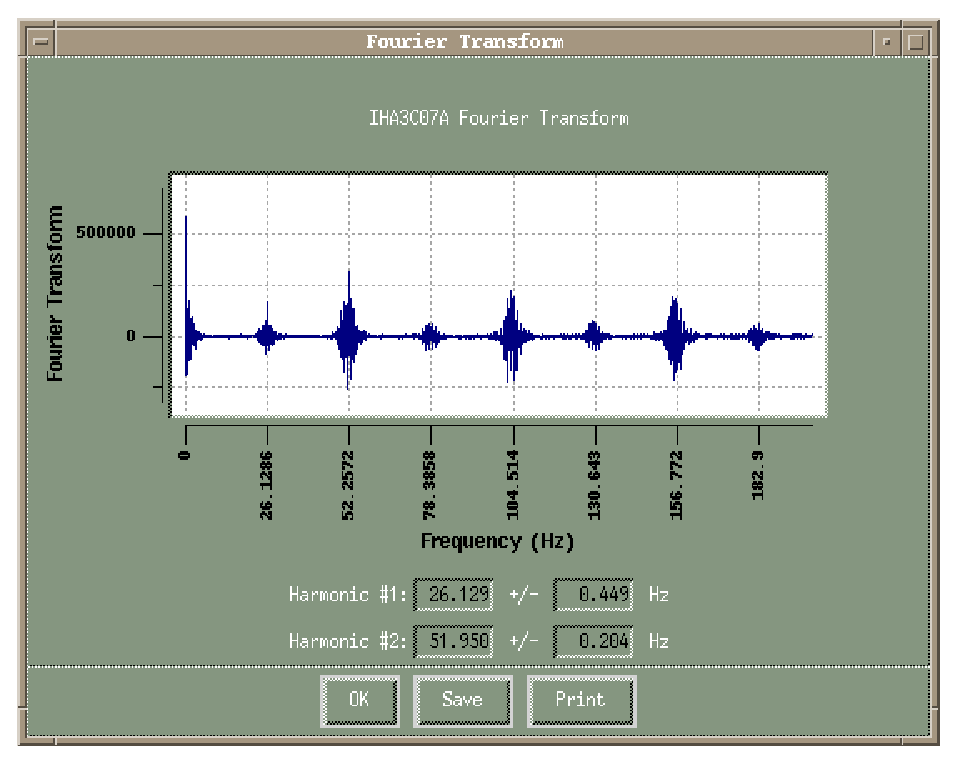
\includegraphics{beamline/fourier_transform.ps}
\caption{The Fourier transform interface.}\label{fig:transform}
\end{figure}
The Fourier transform used to isolate the fundamental frequency of the beam is
\begin{equation}
\hat f(t)=\int_{-\infty}^\infty f(s)\cos \frac{2 \pi s t}{v} {\rm d}x,
\end{equation}
where $v\approx 0.248\mu m/s$ is the speed of the encoder.  Let $N(x)$ be a continuous interpolation of
the harp data, so that $N(x)$ equals the electron count $n_i$ at each of the data points $(x_i, n_i)$ and
0 off the scanning region $(x_{min}, x_{max})$. Then
%\begin{eqnarray}
%\hat N(s)&=&\int_{-\infty}^\infty N(x)\cos \frac{2 \pi s t}{v} {\rm d}x \\
%	&=&\int_{x_{min}}^{x_{max}} N(x)\cos \frac{2 \pi s t}{v} {\rm d}x \\
%	&\approx& \frac{\Delta x}{3}\sum_{i<i_{max}} c_i n_i(x_i) \cos \frac{2 \pi x_i s}{v},
%\end{eqnarray}
%Ed. Note: the above eqnarray was reformatted below for compatibility with latex2html.
\begin{center}
\begin{equation}
\begin{tabular}{rcl}
$\hat N(s)$&$=$&$\int_{-\infty}^\infty N(x)\cos \frac{2 \pi s t}{v} {\rm d}x$ \\
	   &$=$&$\int_{x_{min}}^{x_{max}} N(x)\cos \frac{2 \pi s t}{v} {\rm d}x $\\
	   &$\approx$&$ \frac{\Delta x}{3}\sum_{i<i_{max}} c_i n_i(x_i) \cos \frac{2 \pi x_i s}{v}$,
\end{tabular}
\end{equation}
\end{center}
where $\Delta x=x_{i+1}-x_i,$ $i_{max}$ is an arbitrary large constant, and the $c_i$ are the constants given
by Simpson's integration method.

By Poisson's summation formula, 
\begin{equation}\label{poisson}
\sum_{n=1, 2,\ldots} \hat f(n\omega) =
	\frac{1}{2\omega}\sum_{n=1, 2, \ldots} f\left(\frac{n}{\omega}\right).
\end{equation}
The algorithm used to isolate the fundamental frequency $\omega_0$ of the beam essentially attempts to
maximize the sum (\ref{poisson}).

	\subparagraph{Statistics calculations}

	{\sl Mean and FWHM}

For each superharp scan, the resulting histogram peak centroids are computed using the equation:
%\begin{eqnarray}
%\overline{x}	& = & \frac{\sum \omega_i x_i}{\sum \omega_i}	\\
%\omega_i	& = & \frac{\sqrt{\sum (\Delta n_i)^2}}{n_i} = \frac{\sqrt{\sum n_i}}{n_i} \; ,
%\end{eqnarray}
\begin{center}
\begin{equation}
\begin{tabular}{rcl}
$\overline{x}$&$ = $&$ \frac{\sum \omega_i x_i}{\sum \omega_i}	$\\
$\omega_i    $&$ = $&$ \frac{\sqrt{\sum (\Delta n_i)^2}}{n_i} $\\
              &$ = $&$ \frac{\sqrt{\sum n_i}}{n_i} $\ ,
\end{tabular}
\end{equation}
\end{center}
\noindent
where $n_i$ is the number of counts at the position $x_i$. $\sum n_i$ represents
the total number of events in the selected peak. The beam position is then calculated via:
\begin{equation}
x_{\rm beam} = \overline{x} - x_{\rm survey} \; ,
\end{equation}
where $x_{\rm survey}$ corresponds to the location of each wire if the beam was along the
ideal path inside the beampipe.

The standard deviation (rms) is calculated from the second moment (variance) of the
distribution:
\begin{equation}
M_2 = \sigma^2 =
	\sqrt{\frac{1}{\sum n_i-1}\frac{\sum \omega_i (x_i-\overline{x})^2}{\sum \omega_i}} \; ,
\end{equation}
and the full width at half maximum (FWHM) from:
\begin{equation}
\sigma = \frac{FWHM}{2\sqrt{2ln2}} \; .
\end{equation}

	{\sl Skewness and Kurtosis}

Statistical higher moments $M_n$ are also calculated:
\begin{equation}
M_n = \frac{\sum \omega_i (x_i-\overline{x})^n}{\sum \omega_i} \; , \; {\rm for \; n>2} \; .
\end{equation}
Since the term $1/(\sum n_i-1)$ appears in $\sigma=\sqrt{M_2},$ most statistical calculations
are also normalized.  

The skewness is defined as the measure of the symmetry of a distribution:
\begin{equation}
B_1=\frac{M_3}{M_2^\frac{3}{2}} \; .
\end{equation}
It vanishes for any distribution completely symmetric about its mean (since this forces $M_n$ to 
vanish for odd $n$), and so vanishes for the normal distribution.

The kurtosis is the measure of a distribution's spread about its mean:
\begin{equation}
B_2=\frac{M_4}{M_2^2}-3
\end{equation}
It also vanishes for a normal distribution, since $M_4=3\sigma^2$ and $M_2=\sigma.$

	\subparagraph{Graph Comparisons}

Using survey data, the program isolates the three peaks of the first graph $H_0$ loaded and plots them in the
three lower graph windows.  As subsequent graphs $H_i$ are loaded, the offset
$\overline{x_{H_i}}-\overline{x_{H_0}}$ is calculated over each of those three regions and displayed in the 
upper-right corner of the appropriate graph.  The offsets have the same order and color as the harp names in
the graph legend.
 
When data from both of a pair of harps (e.g. IHA3C17A and IHA3C17B) are loaded, the angle $\theta$ the
beam makes with the horizontal when travelling through the pair is calculated and displayed.  As with the
offsets, the color of the displayed angle matches the color of graph of the harp pair.

\paragraph{Beam energy measurement}\label{energy}

After loading the data from the superharps at the entrance (IHA3C07A and IHA3C07B) and at
the exit (IHA3C17A and IHA3C17B) of the hall C arc beamline, 
the \fbox{Calculate dP/P0} option
will be enabled?  This menu option allows users to calculate the beam incident energy through some
conditions:
\begin{enumerate}
\item If the full width of the first peak of harp IHA3C07A is less than twice the full
width of the first peak of harp IHA3C17A, then the beam is not dispersive enough to perform the
calculation, and an error will be generated.
\item Prior to the calculation, one has to verify the dispersion and the amplification factor at the
exit of the arc related to the hall C beamline optic settings. The default values are now 12.5~cm and 3,
respectively.
\item {\bf Only the MCC operators are allowed to perform the beam energy calculation since there is a setup
procedure to follow~\cite{ebeam_proc99} (see
appendix~\ref{append_ebeam_proc99})}.  The users can
re-evaluate this calculation by asking for the setting current of the arc dipole magnets and loading all
the corresponding superharp data.
\end{enumerate}

The basic idea behind the calculation is as follows.
Suppose a particle with mass $m$ and charge $q$ is subjected to a magnetic field $\vec{B}$ perpendicular
to the plane of the particle's motion, causing it to travel in a circular path of radius $R$. The beam
momentum $P_0$ is determined via:
\begin{equation}
P_0 = \frac{e}{\Theta}\int Bdl
\end{equation}
where $\int Bdl$ is the magnetic field integral over the path of the electron beam and
$\Theta = 34.3^\circ$ is the bending angle through which the electron beam is deflected. $\int Bdl$ is
determined by mapping bending magnets absolutely with a combination of NMR and Hall probes. Taking $e$
as a constant, this leads to the uncertainty relation:
\begin{equation}
\frac{\Delta P}{P_0} = \sqrt{\Big (\frac{\Delta \int Bdl}{\int Bdl}\Big )^{2}
                     + \Big (\frac{\Delta \Theta}{\Theta}\Big )^{2}} \; .
\end{equation}

The inclusion of the beam incident angle is taken into account by utilizing the Lorentz force:
\begin{equation}
\vec{F}=-e\vec{v}\times \vec{B} = m_e\vec{a},
\end{equation}
where $\vec{a}$ is the acceleration and $m_e$ the mass of the electron. Projecting on the three cartesian
axis (z-beam direction, x-transverse horizontal and y-transverse vertical):
\begin{equation}
\left \{
\begin{array}{lll}
a_x & = & -\frac{evB}{m_e} 	\\
a_y & = & 0			\\
a_z & = & 0			\\
\end{array}
\right .
\Leftrightarrow
\left \{
\begin{array}{lll}
v_x & = &  -\frac{evB}{m_e}t + vsin(\theta _x)	\\
v_y & = & vcos(\theta _y)				\\
v_z & = & vcos(\theta _x)				\\
\end{array}
\right .
\end{equation}

\begin{equation}
\Leftrightarrow
\left \{
\begin{array}{lll}\label{eq:txy}
x & = &  -\frac{evB}{2m_e}t^2 + vsin(\theta _x)t + x_0	\\
y & = & vcos(\theta _y)t + y_0				\\
z & = & vcos(\theta _x)t + z_0				\\
\end{array}
\right .
\end{equation}
We are in a case where: $z_0 = 0$. Therefore:
\begin{equation}
\left \{
\begin{array}{lll}
t & = & \frac{z}{vcos(\theta_x)}					\\
x & = & -\frac{eB}{2m_evcos^2(\theta _x)}z^2 + tan(\theta _x)z + x_0	\\
y & = & \frac{cos(\theta _y)}{cos(\theta _x)}z + y_0			\\
\end{array}
\right .
\end{equation}
The system in (\ref{eq:txy}) characterizes the trajectories of the particle along
$x$ and $y$ as a function of its position inside the magnetic region along $z$.

The expression of $x$ represents the trajectory of the particles in the dispersion plane
(where the particles are subject to the magnetic field):
\begin{equation}
x = -\frac{eB}{2Pcos^2(\theta _x)}z^2 + tan(\theta _x)z + x_0,
\end{equation}
where $x = x_{17}$, $x_0 = x_{07}$ and $\theta _x = \theta _{07}$ are determined by using the superharps
at the entrance (IHA3C07) and at the exit (IHA3C17) of the arc. The beam momentum $P$ corrected from
incident beam angle can then be evaluated.

\paragraph{Further Help}

For further assistance, contact
\par
\noindent
\begin{table}[!ht]
\begin{tabular}{l}
Paul Gu\`eye \\
e-mail: {\tt gueye@jlab.org} \\
Phone: (757) 269-7167 \\
Pager: (757) 849-7167 \\
\end{tabular}
\end{table}



\subsection{M\o ller Polarimeter }
The M\o ller Polarimeter is used to measure the electron beam
polarization. Instructions for carrying out such a measurement
are documented in a 
\htmladdnormallinkfoot{Step-by-Step Guide}{http://www.jlab.org/Hall-C/document}.
MCC follows a complementary 
\htmladdnormallink{procedure}{http://opsntsrv.acc.jlab.org/ops_docs/online_document_files/MCC_online_files/HallC_Moller_pol_measurement_proc.pdf}.
The polarimeter is located at the beginning of the Hall C
alcove downstream of the granite table that holds the super-harps.
All magnetic elements of the polarimeter are located between
the BPMs 3C17 and 3C18: there are a solenoid and two quadrupoles.
The M\o ller target is located in the center of the solenoid. The
detectors are positioned 11 meters downstream of the target and 0.49
meters away from the beam line in a lead house.

The Hall~C M\o ller polarimeter consists of: the target and target solenoid, the quadrupole magnets, a 
collimator box, and the detectors.  These are described in turn in 
the paragraphs below:

{\sl Target Solenoid} This is a $\approx$ 3 T super conducting
solenoid used to ``brute force" polarize the valence electrons in a
thin, $\approx$ 10 $\mu$m, iron foil perpendicular to the
plane of the foil. This magnet has a liquid nitrogen cooled radiation shield
and requires liquid helium for operation.

{\sl Quadrupole Magnets} In order to keep the locations of the M\o ller
target and detectors fixed regardless of the incident beam energy
a two quadrupole optics was chosen. The first quadrupole (``the Los Alamos Quad")
has a 4 inch bore and a physical length of about 1 ft.
The second quadrupole (10Q36) has a 10 inch bore and physical length of 123 cm.

{\sl Collimator Box} There are seven movable blocks of densimet (densimet is
a machinable alloy of tungsten) for the collimator. These blocks form two
horizontal jaw pairs and one vertical jaw pair. The seventh block has a
hole in it through which the unscattered electron beam travels.

{\sl Detectors} The Hall~C polarimeter was built to operate in coincidence
mode with both the scattered and recoiling electrons being detected in
coincidence. There are thus two identical detector stacks placed symmetrically
about the beamline. Each stack consists of a sixteen element hodoscope
followed by a lead glass block.

\paragraph{Polarimeter Description}
The layout of the polarimeter is shown in fig.~\ref{polscetch}.
The incoming electron beam hits an iron target foil. The target thickness
is on the order of 4 to 10 $\mu m$. The electrons in the iron foil
are polarized by the 3 T magnetic field of the super conducting solenoid.
The beam electrons scatter off 
the target electrons (M\o ller Scattering) 
with the scattering angle of interest at about
1$^{\circ}$ or below in the laboratory system. Since the electrons
are very close to the beam line they need to be deflected away from
it in order to be detected in coincidence. This is achieved by
two quadrupoles. The first smaller quadrupole is focusing in the
horizontal plane  while the
second large quadrupole is defocusing in the same plane. The use of two quadrupoles
allows us to keep the cone of the 90$^{\circ}$ CM scattered electrons 
at fixed dimensions after a 11 meter drift distance, namely
49cm horizontal and 16cm vertical from the beam line.
The first quadrupole (the Los Alamos Quad) has a 4 inch bore and a
physical length of 12 inches. The second quadrupole (10Q36) has a 10
inch bore and a physical length of 123 cm.
\begin{figure}[htp]
\begin{center}
\includegraphics[height=4in,width=6in]{beamline/polarimeter.eps}
\caption{Sketch of the M\o ller polarimeter in Hall C.\label{polscetch}}
\end{center}
\end{figure}
The two electrons are detected in coincidence using two lead glass 
shower counters as shown in Figure \ref{detarr}. In front of each counter is a collimator that defines
the acceptance. The right collimator is intentionally larger
than the left. This reduces the sensitivity of the coincidence 
acceptance to beam and detector positions. In front of the collimator
is a hodoscope with 16 channels. Each channel is a scintillator of 1cm
width.
\begin{figure}
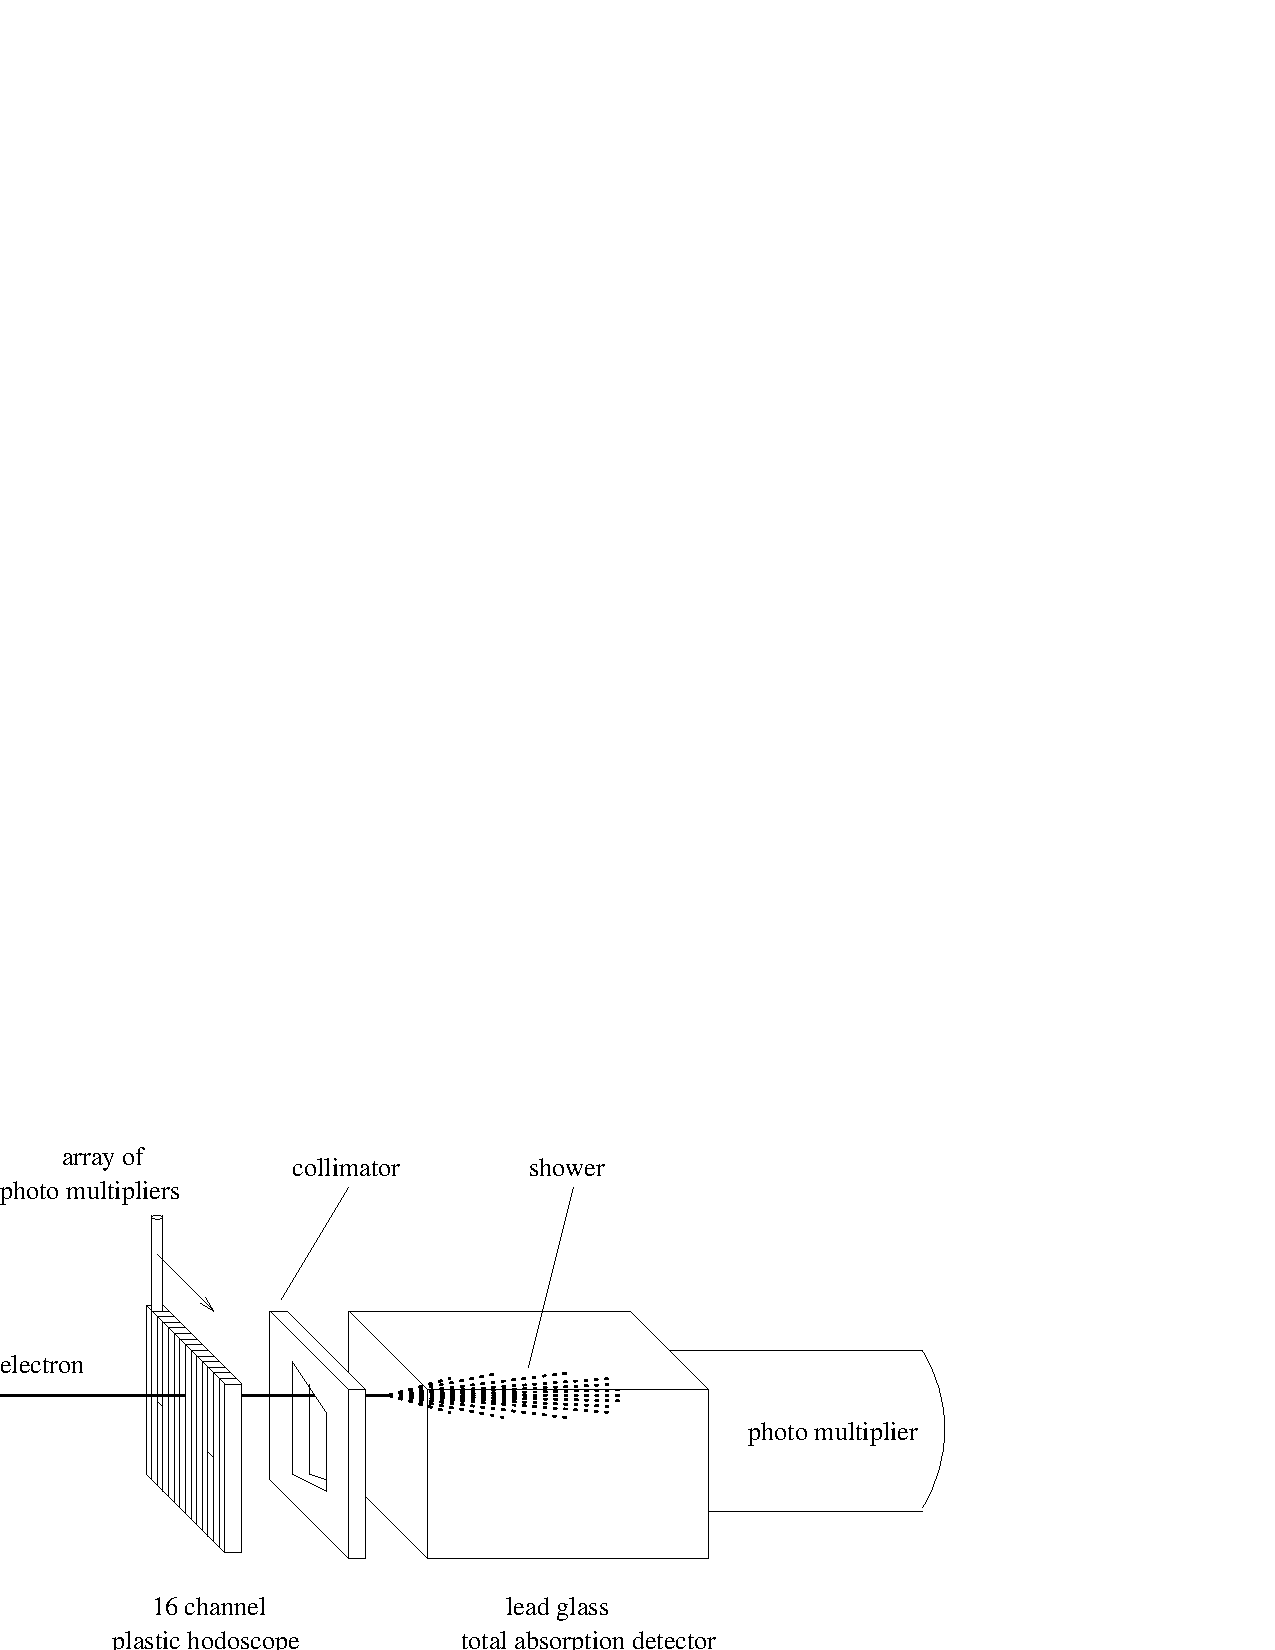
\includegraphics[height=4in,width=6in]{beamline/detarangement.epsf}
\begin{center}
\parbox{10cm}{
\caption{Detector arrangement}\label{detarr}}
\end{center}
\end{figure}

Since the cross section for Mott scattering (electron - nucleus
scattering) is much larger than M\o ller scattering it is necessary
to use collimators to reduce this background that leads to accidental
coincidences. This is achieved with a set of movable collimators
located between the two quadrupoles (see fig.~\ref{polscetch} 
and \ref{colscetch}). 
%
\begin{figure}
\includegraphics[height=4in]{beamline/collim.eps}
\begin{center}
\caption{Collimator with M\o ller trajectories\label{colscetch}}
\end{center}
\end{figure}
Mott electrons with the right momentum and scattering angle that make it
through the quadrupoles into the detectors do not follow the same
path in configuration space as 
the M\o ller electrons do.  The collimators are used to shield the
space that is not transversed by the M\o ller electrons. The space of
the M\o ller stripes is  
given by the collimators in front of the lead glass detectors
that define the coincidence acceptance.
%

\paragraph{M\o ller Control Software and Hardware}
There are three main control packages for the M\o ller Polarimeter.
Two of them are GUIs run from the Hall C Counting Room. They
control 1)~the solenoid cryogenics, and 2)~the solenoid field, 
the target, and the collimators. Control of the two quadrupoles
is possible only from MCC, although the second counting room GUI does
allow experimenters to monitor the quadrupole settings.


\begin{figure}
  \begin{center}
%  \htmlimage{scale=1.0,thumbnail=0.5}
  \includegraphics[height=4in]{beamline/mollergui.ps}
  \caption{M\o ller Polarimeter Control GUI\label{molpolmedm}}
  \end{center}
\end{figure}
%

\subparagraph{Polarimeter GUI}

To run the GUI using medm do the following steps
\begin{itemize}
\item Log onto cdaqh1 from the account {\tt cvxwrks}.
\item Set directory: \begin{verbatim} cd MEDM/moller \end{verbatim}
\item Start the GUI: \begin{verbatim} medme moller.adl  \end{verbatim} 
\end{itemize}
%

\subparagraph{Quadrupole Settings}

Although the quadrupoles are controlled only by MCC, it is the 
responsibility of the experimenter to make certain that they are
set to the correct currents.
The correct currents are a function of the incidentbeam energy . The example currents given in Table \ref{tab_qcurrent} are in Amps
and were determined by tuning the system using beam. The final currents 
are determined experimentally by optimizing the
M\o ller hodoscope left-right correlation. This guarantees that the polarimeter
acceptance is centered around 90 degrees in the center of mass.
%
\begin{table}[!hbt]
\begin{center}
\begin{tabular}{|c|c|c|l|} \hline
Beam Energy & Q1  & Q2 &Reference data \\
\hline
0.884 &  85.9 & 112.0 & March, 2001  \\
2.332 & 136.0 & 364.0 & August, 2001 \\
2.415 & 137.1 & 380.0 & April, 2001  \\
3.395 & 142.2 & 586.0 & March, 2001  \\
\hline 
\end{tabular}
\caption{M\o ller Quadrupole Current Setings\label{tab_qcurrent}}
\end{center}
\end{table}

A reminder to the expert: After a power failure or power cycle of the Q1 
power supply and/or controller,
it is necessary to press the green "START" button on the Q1 (Small
M\o ller Quad) power supply.  If MCC cannot get any real current out of the
supply then probably it is in standby mode and needs the START button pushed.

Currently the Degauss procedure for Q2 is to ramp the magnet up to 800 Amps 
then ramp down to zero, reverse polarity, ramp to -240 Amp and finally
back to zero. This procedure is almost never used and is not known to
be important.

%
\subparagraph{Target Motion}
There are four possible target positions, shown in Table \ref{tab_moltar}. They
can be selected using the GUI  
with the frame title {\tt ``Target Ladder''} . In the menu indicated
by the term {\tt ``Cancel''} the four individual target positions 
can be selected. Once chosen with the mouse pointer the 
target ladder will move! {\bf ALWAYS (BEAM OFF) WHEN TARGET IS BEING MOVED.}
Since the target positions are hardwired in the code, any 
corrections to these values need to be done manually using 
the {\tt ``Jog''} option of the GUI. The camera button {\tt ``ON OFF'' }
turns  the target camera and light on and off respectively.
\begin{table}
\begin{center}
\begin{tabular}{|c|c|c|l|c|} \hline
Target & Material & Thick $mu$m & State & Position \\
\hline
1 & Fe & 4  & polished   & -1.96   \\
2 & Fe & 10 & polished   & -0.48  \\
3 & Fe & 4  & unpolished & +1.00  \\
4 & Fe & 10 & unpolished &  n/a \\
\hline 
\end{tabular}
\parbox{10cm}{
\caption{M\o ller Targets\label{tab_moltar}}}
\end{center}
\end{table}
%
After a power cycle the target first needs to find HOME. This can
be done selecting the {\tt ``HOME''} in the menu. To move the target
ladder fully out of the beam select  {\tt ``RETRACT''} from the menu.
At position -3.86 the target is fully out of the beam.
%
\subparagraph{Collimator Positions}
{\bf Never move collimator 5 while beam is present!!!}\\
{\bf Never issue the Go Home while beam is present!!!}\\
The collimator positions also depend on beam energy. However
this dependency is only small since the collimators do not need
to be located very tight to the M\o ller stripes. The singles rates 
do not increase significantly if the collimators are even 5 mm away 
from the M\o ller stripes. The menu in the GUI for the collimator
control provides three different predefined collimator settings.
These settings can be loaded and executed or the values
can be typed in manually.

Each collimator can be moved individually be typing a value in the 
column {\tt ``SetPoint''}
at the appropriate window, see fig. \ref{molpolmedm}. Use the {\tt ``RETURN''} key
to set the value and the {\tt ``Move''} button to move the collimator
to this value. For the collimators 1,2,3,4,6 the values can not 
be larger than zero because that would move the collimators into the
beam (software cut). The collimator 5 is a special case since the beam goes through
a central hole in the collimator. 
After a power cycle all the collimators need to find the HOME position
first.  This is done by using the {\tt ``Go Home''} menu that pops up
a window to ask if one really want to search the home position. 
%
\subparagraph{Target Solenoid}
Since the target solenoid is super conducting and therefore cooled
with liquid helium the console is somewhat more complicated.
Currently we run the magnet at a field of 3 Tesla. Before ramping
up the magnet, check the helium and nitrogen levels
(see fig \ref{molpolmedm}). The magnet has to be put 
into standby mode first, this turns the heater on.  Use button {\tt ``SDBY''}. 
After 20 seconds one
can ramp up the magnet using the {\tt ``GO SET''} button. This ramps up
the magnet to the field value set in the frame {\tt ``Set Field(Tesla)''}.
After reaching the desired field the magnet can be put into persistent mode 
(i.e. turns off the heater) by hitting the button {\tt ``PRST''}. 
The maximum ramp up speed is 12 Amps per minute. 
However, the first ramp-up after a thermal cycle should be made at
6~amps/minute up to 2.4~T, followed by 3~amps/minute to 3~T.
The power supply has an internal ramp up parameter
that will limit ramping to 4 Amps per minute at higher fields.
The ramp up process can be stopped at any time by hitting the {\tt
``HOLD''} button. \\ \\
After a power cycle the remote button {\tt ``REM''} has to be activated
first in order to establish communication to the power supply.
The power supply is an IPS120-10 from OXFORD. Since it is a polarity
reversible device the sign of the field value chosen by the
{\tt ``Set Field(Tesla)''} is important. To reverse polarity the magnet
needs to be ramped down to zero first.
%


\newpage
\subparagraph{M\o ller Cryogenics GUI}
The liquid nitrogen and helium supplies are monitored and controlled by
a GUI with the drivers running on the IOC vmec10 (aka {\it iochc10}).
A screen snapshot is shown in Figure \ref{molcryomedm}.
To run the GUI using medm, perform the following steps:
\begin{itemize}
\item Log onto cdaqh1 from the account {\tt cvxwrks}.
\item Set directory: \begin{verbatim} cd MEDM/Moller/CRYO \end{verbatim}
\item Start the GUI: \begin{verbatim} medme hcmcryo.adl  \end{verbatim} 
\end{itemize}

\begin{figure}
\begin{center}
\includegraphics[height=4in]{beamline/molcryogui.ps}
\caption{M\o ller Cryo GUI\label{molcryomedm}}
\end{center}
\end{figure}
%

Normally, the cryogen levels in the solenoid cryostat should be
automatically maintained at or above 60\% by the controls software.
If mandated, you may turn off the supply of helium or nitrogen by
closing JT-valves {\tt EV91017} or {\tt EV91018}, respectively.

Note that if VMEC10 (iochc10) gets rebooted, it is necessary to RESTORE the cryo valve
parameters for the M\o ller. You do this by clicking on the small blue box on the
bottom of the cryo overview screen (hcmcryo.adl), selecting "SAVE/RESTORE",
then selecting "iochc10:NORMAL RESTORE" from the "!" box in the resulting
screen. It will prompt you to hit ENTER several times. Do so until the dialog
window goes away.

Cooling down the magnet from room temperature should only be done
by a M\o ller cryo expert. The steps are
\begin{enumerate}
	\item Close {\tt EV91019} to isolate the cold return line.
	\item Open {\tt EV91018} to about 35\% and flow nitrogen at this rate
		until the nitrogen level indicator shows liquid in the cryostat.
		This may take several hours. (You may start precooling the helium
		lines [below] at the same time.)
	\item Using the submenu pushbutton for {\tt EV91018}, put the valve on
		PID control. PID parameters should be:
	\begin{enumerate}
		\item Max Pos = 35.0
		\item Min Pos = 7.0
		\item Max Chg = 15.0
		\item Min CHg = 0.1
		\item Set Val = 90.0
		\item ST = 60.0
		\item Gp = 1.0
		\item Gi = 0.025
		\item Gd = 0.0
	\end{enumerate}
	\item Observe that the nitrogen level now controls the position of {\tt EV91018}.
	\item pre-cool the helium lines by opening {\tt EV91001} to 100\% and
		opening {\tt EV91017} as much as possible without exceeding the total
		Hall-C 4K helium consumption limit. Monitor the flow and 
		reduce {\tt EV91017} as the system cools down (the flow will 
		increase as the system temperature nears 4K).
	\item When the cryostat helium level indicator shows 50\% or higher, put
		{\tt EV91017} on automatic control. The supply JT valve is controlled 
		such that both the liquid level and the supply temperature are maintained
		at reasonable values. The standard PID parameters are shown in 
		figs.~\ref{fig:ev17c}, \ref{fig:ev17llc} and~\ref{fig:ev17stc}.
	\item The system is now in automatic control with {\it Warm Return}. Normally it
		runs in {\it Cold Return}, which is much more energy efficient. Procedures
		for transitioning to {\it Cold Return} will be forthcoming. Until they
		are approved for non-expert use, contact Paul Brindza to switch the
		system to {\it Cold Return}.
\end{enumerate}

\begin{figure}[h!]
\begin{latexonly}
\centering
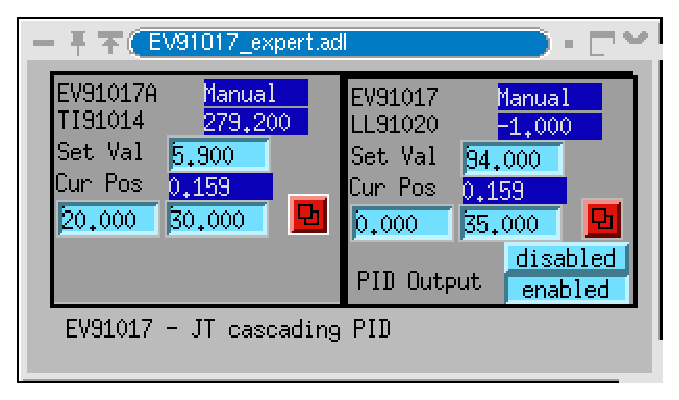
\includegraphics[width=3in]{beamline/ev91017_cascade.eps}
\caption{PID MEDM Screen - EV91017 Cascade Loop}
\label{fig:ev17c}
\end{latexonly}
%----------------------------
\begin{htmlonly}
\htmlimage{scale=1.0}
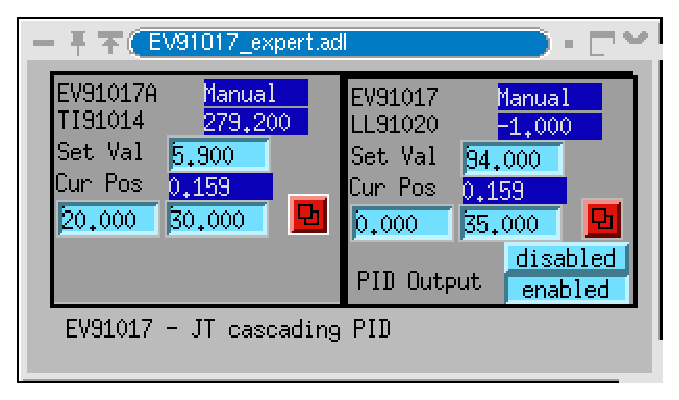
\includegraphics{beamline/ev91017_cascade.eps}
\caption{PID MEDM Screen - EV91017 Cascade Loop}
\label{fig:ev17c}
\end{htmlonly}
\end{figure}


\begin{figure}[h!]
\begin{latexonly}
\centering
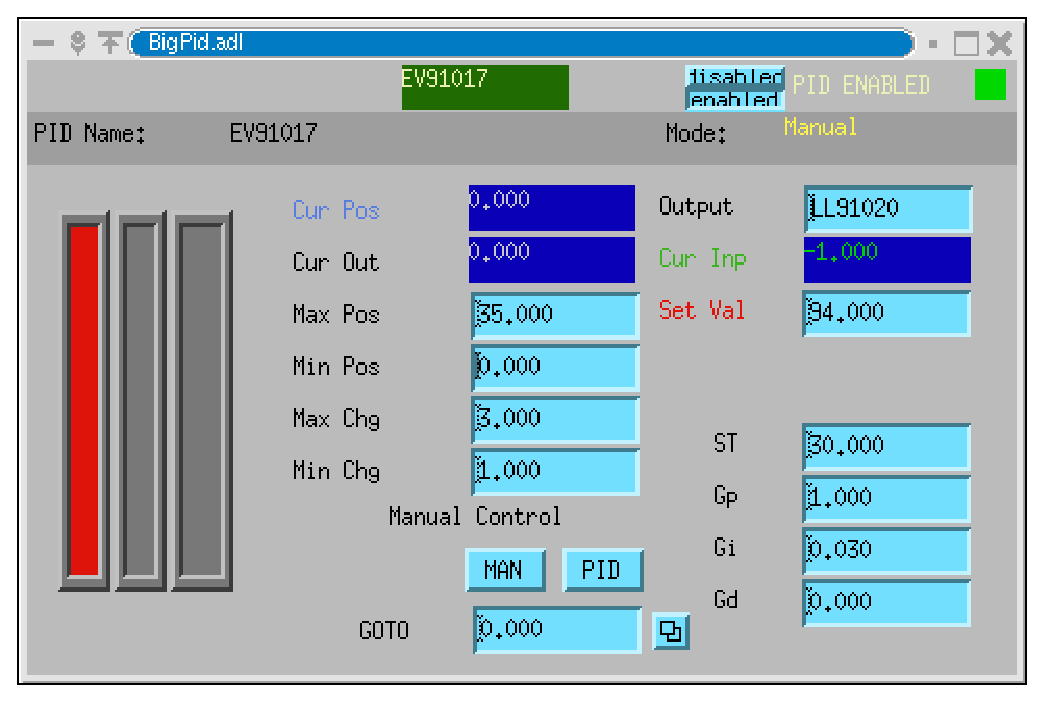
\includegraphics[width=3in]{beamline/ev91017.eps}
\caption{PID MEDM Screen - EV91017 Liquid Level Control}
\label{fig:ev17llc}
\end{latexonly}
%----------------------------
\begin{htmlonly}
\htmlimage{scale=1.0}
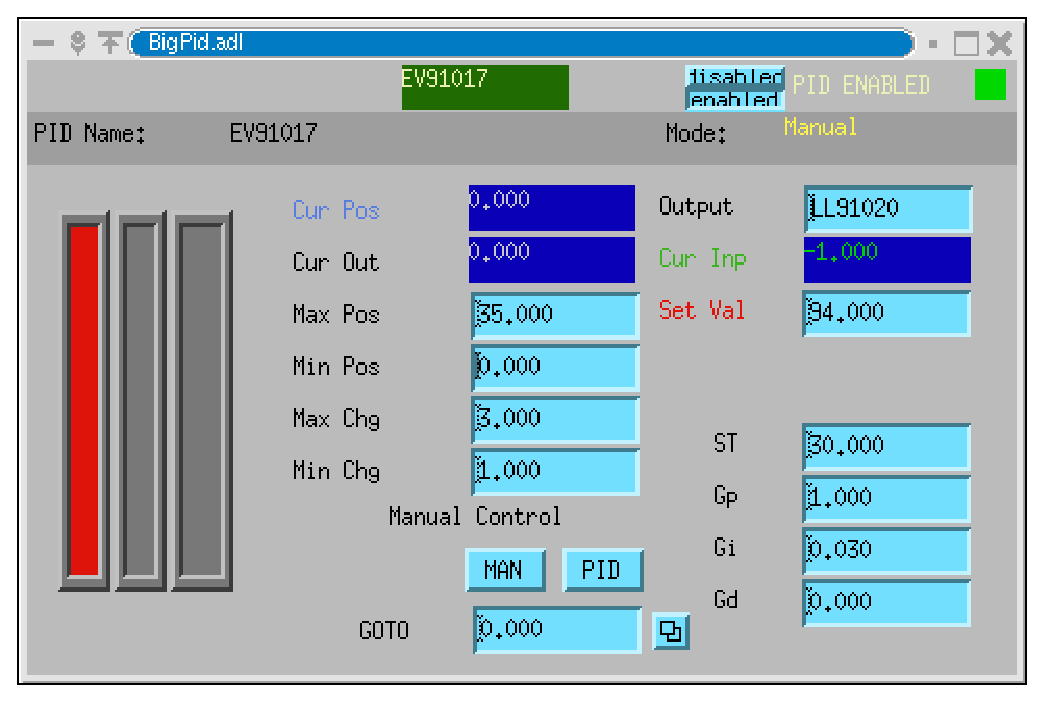
\includegraphics{beamline/ev91017.eps}
\caption{PID MEDM Screen - EV91017 Liquid Level Control}
\label{fig:ev17llc}
\end{htmlonly}
\end{figure}


\begin{figure}[h!]
\begin{latexonly}
\centering
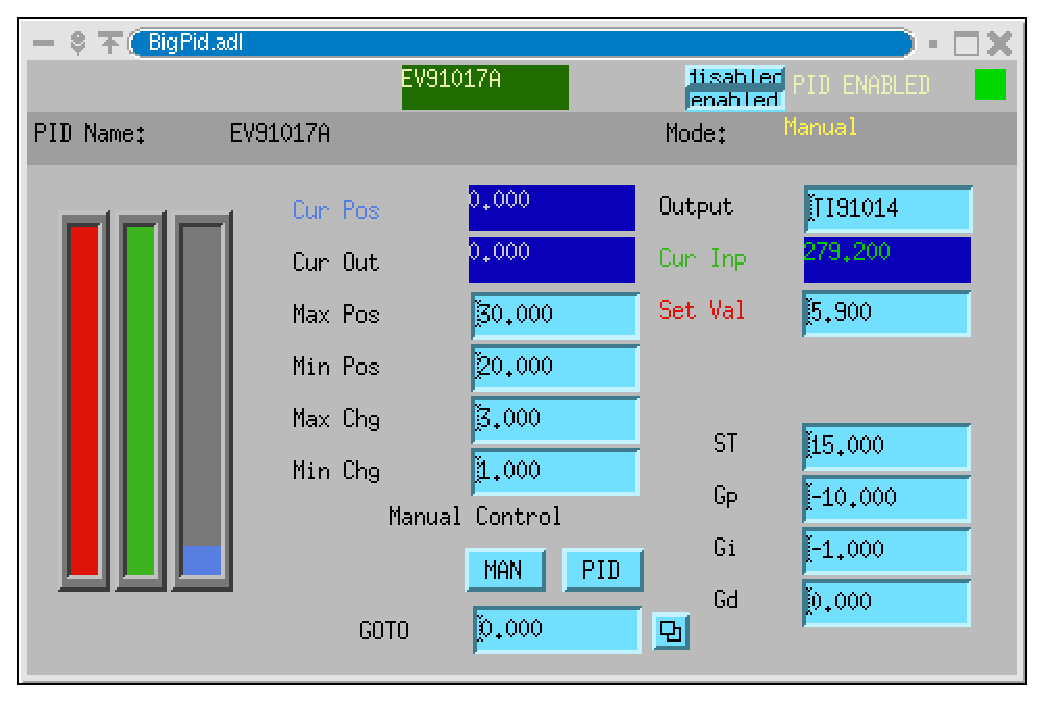
\includegraphics[width=3in]{beamline/ev91017a.eps}
\caption{PID MEDM Screen - EV91017 Helium Supply Temperature Control}
\label{fig:ev17stc}
\end{latexonly}
%----------------------------
\begin{htmlonly}
\htmlimage{scale=1.0}
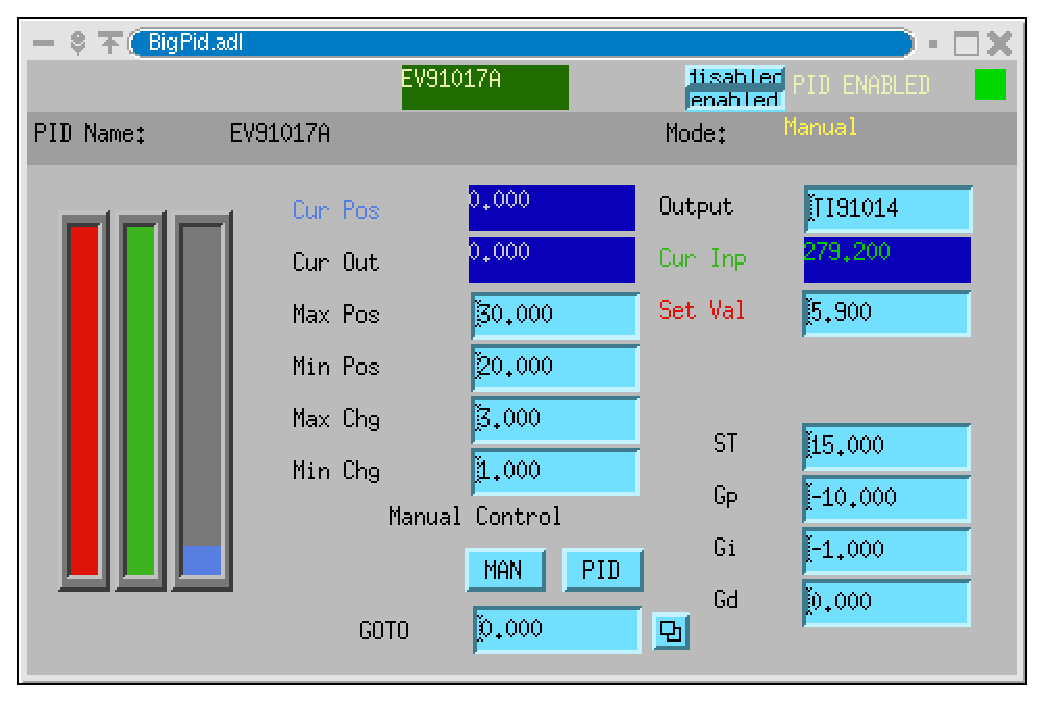
\includegraphics{beamline/ev91017a.eps}
\caption{PID MEDM Screen - EV91017 Helium Supply Temperature Control}
\label{fig:ev17stc}
\end{htmlonly}
\end{figure}




\subparagraph{Detector HV}
The HV of all detectors is controlled from the SOS HV
GUI. Nominal settings for the PMT's are given in Table~\ref{tab:mol_hv}.
If necessary, the M\o ller High Voltages can be controlled from the front panel
of the CAEN mainframe from which they are powered. This mainframe is the only
one in relay rack CHC15.
\begin{table}
\begin{center}
\caption{Nominal M\o ller Detector High Voltages and CAEN Power Supply Assignments\label{tab:mol_hv}}
\vspace{\baselineskip}
\begin{tabular}{|l|c|c|c|c|}
\hline
{}         & {}   & {}    & {}    & {}    \\
Detector   & Left & Left  & Right & Right \\
           & HV   & CAEN$\#$ & HV    & CAEN$\#$ \\
{}         & {}   & {}    & {}    & {}    \\ \hline
Pb Glass   & 1220* & 38   & 1310* & 39    \\
Hodo 01    & 1200  & 00   & 1220  & 05    \\
Hodo 02    & 1220  & 01   & 1190  & 06    \\
Hodo 03    & 1150  & 02   & 1120  & 07    \\
Hodo 04    & 1190  & 03   & 1100  & 08    \\
Hodo 05    & 1100  & 04   & 1120  & 09    \\
Hodo 06    & 1120  & 10   & 1200  & 15    \\
Hodo 07    & 1150  & 11   & 1100  & 16    \\
Hodo 08    & 1080  & 12   & 1270  & 17    \\
Hodo 09    & 1230  & 13   & 1100  & 18    \\
Hodo 10    & 1100  & 14   & 1180  & 19    \\
Hodo 11    & 1250  & 20   & 1150  & 25    \\
Hodo 12    & 1230  & 21   & 1200  & 26    \\
Hodo 13    & 1160  & 22   & 1150  & 27    \\
Hodo 14    & 1200  & 23   & 1180  & 28    \\
Hodo 15    & 1220  & 24   & 1170  & 29    \\
Hodo 16    & 1200  & 30   & 1150  & 35    \\
\hline
\end{tabular}
\end{center}
\end{table}
*{\it Note: The lead-glass voltages are beam energy dependent.}

\subparagraph{M\o ller IOCs Reference}

There are two IOCs which support the polarimeter devices. One
(iochc10 or {\it vmec10}) is on the Hall~C network and under the
control of Hall~C staff. It manages the superconducting solenoid
power supply and cryogenics system as well as the M\o ller target and
collimators. The other IOC (iochc11) is {\tt owned} by MCC. It
operates the two M\o ller quadrupoles. Software running on both
IOCs is maintained by the accelerator software group.

M\o ller quadrupoles Q1 and Q2 are controlled by the same IOC.
The power supply for Q2 communicates over GPIB. This requires a 
CPU board MV167 with an industry pack (IP)
for GPIB interface together with a HiDEOS board MV162 since EPICS
does not support GPIB directly. The CPU is called iochc11 (it had
been known as vmec11 prior to September 2001) and
is located in the right-hand half of a split backplane VME crate 
downstairs in the hall behind the green
shielding blocks. The EPICS drivers are located on the opsrv cluster.
The boot ROM looks as follows:

\begin{verbatim}
boot device          : ei 
processor number     : 0 
host name            : opsrv 
file name            : /cs/op/iocs/iochc11/vx/vxWorks 
inet on ethernet (e) : 129.57.242.11:fffffc00 
inet on backplane (b): 
host inet (h)        : 129.57.236.50 
gateway inet (g)     : 129.57.240.1 
user (u)             : vxwrks 
ftp password (pw) (blank = use rsh): 
flags (f)            : 0x0 
target name (tn)     : iochc11
startup script (s)   : /cs/op/iocs/iochc11/startup 
other (o)            : 
\end{verbatim}


The M\o ller target, collimators, solenoid power supply, and
solenoid cryogenics controls are all handled by vmec10 (also
known as iochc10) which resides in the left-hand side of the
same split backplane VME crate. Its boot ROM looks like:

\begin{verbatim}
boot device          : ei 
processor number     : 0 
host name            : opsrv 
file name            : /cs/op/iocs/iochc10/vx/vxWorks 
inet on ethernet (e) : 129.57.168.110:fffffc00 
inet on backplane (b): 
host inet (h)        : 129.57.236.50 
gateway inet (g)     : 129.57.168.1 
user (u)             : vxwrks 
ftp password (pw) (blank = use rsh): 
flags (f)            : 0x0 
target name (tn)     : iochc10 
startup script (s)   : /cs/op/iocs/iochc10/startup 
other (o)            : 
\end{verbatim}




%
\paragraph{Data acquisition}
The data acquisition reads out three Struck scaler modules at each
(possible) helicity transition. Scalers '1' and '2' are gated for '+'
and '-' helicity intervals as defined by the signal coming from
MCC. (For experiments using delayed helicity reporting the active
scaler will still be determined by the MCC signal, but this signal
does not necessarily indicate the instantaneous helicity state. The
actual state must be determined at analysis time.) Scaler '3' is gated
'on' during all helicity intervals, and should normally count the sum
of scalers '1' and '2'.

The CAMAC Crate is read out
on an prescaled event by event basis reading one ADC and one TDC
module and two dual port memories. The ADC and TDC provide diagnostic
information about the lead glass shower counters and the
M\o ller coincidence timing. The memories provide horizontal 
positioning information about the two M\o ller electrons in front
of the shower counters. This information is used to optimize
the quadrupole settings in order to center the 90$^{\circ}$ CM
M\o ller electrons on the lead glass. \\ \\
Data is taken using CODA2.1 running on cdaqs1. The run type
is Moller21 and can be started from the same location as the
main experiment.

\paragraph{M\o ller Beam line tuning}

A thorough step-by-step procedure for tuning the beam through the
polarimeter has been worked out with the MCC operations group. Only
MCC operators may modify the settings of the two M\o ller quadrupoles.
The procedure is available for your reference at
\htmladdnormallink{http://opsntsrv.acc.jlab.org/ops\_docs/online\_document\_files/MCC\_online\_files/HallC\_moller\_pol\_measurement\_proc.pdf}{http://opsntsrv.acc.jlab.org/ops_docs/online_document_files/MCC_online_files/HallC_moller_pol_measurement_proc.pdf}. In addition, there is a companion 
document for Hall-C operators to follow. It is available in print form in
the counting room, or on the web at 
\htmladdnormallink{Hall-C Moller Step-by-Step Guide}{http://www.jlab.org/Hall-C/document/manuals.html}.

The following is simply a coarse outline of the steps to be followed.
For actually tuning up the beamline and turning on the polarimeter, you {\bf must}
refer to the separate documents mentioned above. The tuneup procedure should take no
more than about 20 minutes if the beam is already tuned to Hall~C.
The time required to ramp up the superconducting solenoid is about 10 minutes.
\begin{enumerate}
        \item With all M\o ller magnets off MCC will
           center  the beam through the BPMs at 3C17  in both
           horizontal  and vertical  directions. 

        \item MCC will then turn on Q1, re-center the beam, then turn
	on Q2 and re-center the beam again. The required quad currents
	must be supplied by Hall~C.  (The M\o ller expert should have
	posted them in the logbook.)

        \item MCC will request that the Hall shift crew ramp up the
	M\o ller solenoid. We normally run it at 3~Tesla.

        \item With the solenoid and the two quadrupoles Q1 and Q2 on
              at nominal current, MCC will once again center the beam
              through the polarimeter and into the hall.

	\item If it is desired to take M\o ller measurements at beam currents
	      higher than $\approx$ 2 $\mu$ A it will be necessary to energize
	      the M\o ller raster system. See the documentation in
              \begin{verbatim} ~cdaq/documents/beamline/Moller_Raster_Manual.txt \end{verbatim}
\end{enumerate}

